\documentclass[8pt]{article}

\usepackage[utf8]{inputenc}

\usepackage{amsmath, bm}
\usepackage{graphicx}
\usepackage{amssymb}
\usepackage{float}
\usepackage{caption}
\usepackage{subcaption}
\usepackage{esint}
\usepackage{tikz}
% set font size to 11pt

% set margin
\usepackage[margin=1in]{geometry}

\usetikzlibrary{calc}
\usetikzlibrary{angles,quotes} % for pic
\usetikzlibrary{patterns,snakes}
\usetikzlibrary{arrows}
\tikzset{>=latex} % for LaTeX arrow head

\setlength{\parskip}{\baselineskip}%
\setlength{\parindent}{0pt}%
\setlength{\headsep}{5pt}

% Define the CG symbol style
\tikzset{
    cg/.style={
        draw,
        circle,
        thick,
        minimum size=0.2cm, % Adjust the size of the circle
        inner sep=0,      % Remove extra padding
        append after command={
            \pgfextra{
                \draw[thick] (\tikzlastnode.south) -- (\tikzlastnode.north);
                \draw[thick] (\tikzlastnode.west) -- (\tikzlastnode.east);
            }
        }
    }
}


\begin{document}

\title{Review of Hanson's Helicoidal surface theory}
\author{lwp26}
\date{December 2024}
\maketitle

\section{Introduction}

\section{Hansons Helicoidal Surface Theory}

% nomenclature
\begin{table}[H]
    \centering
    \begin{tabular}{c l}
        \hline
        Symbol & Description \\
        \hline
        $r_t$ & tip radius of the propeller \\
        $r$ & distance from origin to observer point \\
        $r_0$ &  radius of source point on blade \\
        $\mathbf{x}$ & observer coordinates $(x_1, x_2, x_3)$ \\
        $\mathbf{y}$ & source coordinates $(y_1, y_2, y_3)$ \\
        $j$ & imaginary unit \\
        \hline
    \end{tabular}
    \caption{Nomenclature}
    \label{tab:nomenclature}
\end{table}

The starting point is Goldsteins version of the acoustic analogy \cite{goldstein_aeroacoustics}.

\begin{equation}
    \rho'(x, t) = -\frac{1}{c_0^2} \int_{-T}^T \int_{S(\tau)} \left( \rho_0 V_n \frac{\partial G}{\partial \tau} + f_i \frac{\partial G}{\partial y_i} \right) dS(y) d\tau
    + \frac{1}{c_0^2} \int_{-T}^T \int_{V(\tau)} T_{ij} \frac{\partial^2 G}{\partial y_i \partial y_j} dy d\tau
    \label{eq:goldstein}
\end{equation}

"It is an exact result. It applies to any
region $V(\tau)$ which is bounded by impermeable surfaces $S(\tau)$
in arbitrary motion provided the source distributions $T_{tj}$ and
$f_i$ are localized enough to ensure convergence of the integrals."

$V_n$ is the surface normal velocity which will be called the monopole term depite
the fact that it behaves like higher order terms when in motion \cite{goldstein_aeroacoustics}.

The dipole source term $f_i$ is the $i$th component of force exerted on the boundary by the fluid.
The quadrupole is the stress tensor $T_{ij}$ which is neglected for simplicity.

Greens function G for the free space wave equation is given by

\begin{equation}
    G = \frac{\delta(t - \tau - R/c_0)}{4\pi R}
\end{equation}
Where $R = |\mathbf{x} - \mathbf{y}|$ is the distance between the source and observer points.

For a stationary drone propeller it is convenient to replace the Cartesian source coordinates to be in the propeller plane.
This is done with the helicoidal coordinates $(\gamma_0, \xi_0, r_0)$.

\begin{align}
    y_1 &= \frac{\Omega r_0 \xi_0}{U} = \xi_0\\
    y_2 &= r_0 \cos \left( \frac{\Omega \gamma_0}{U} \right) \\
    y_3 &= r_0 \sin \left( \frac{\Omega \gamma_0}{U} \right)
\end{align}

\begin{equation}
    R = \sqrt{ \left( x -  \frac{\Omega r_0 \xi_0}{U}\right) + y^2 + r_0^2 - 2yr_0\cos\left( \frac{\Omega \gamma_0}{U} \right)}
    \label{eq:R}
\end{equation}

\begin{figure}[H]
    \centering
    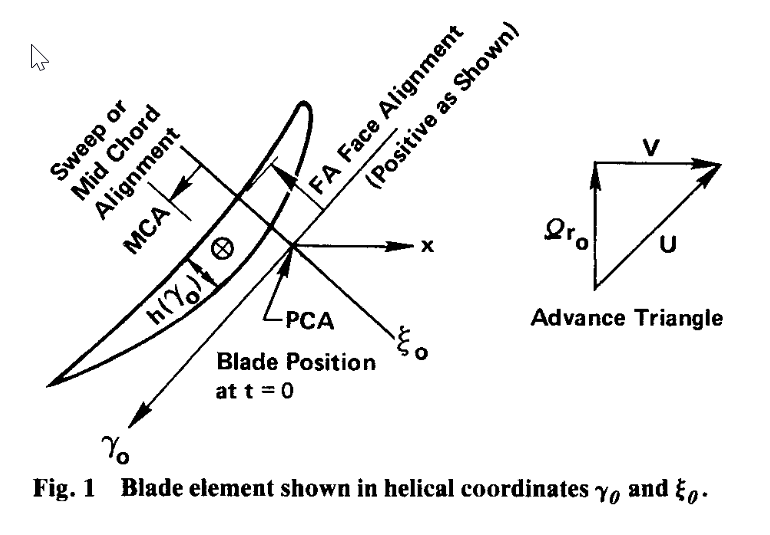
\includegraphics[width=0.4\textwidth]{hansonfoil.png}
    \caption{Local section of propeller blade for Hansons theory}
    \label{fig:bem_section}
\end{figure}

In the following section thin airfoil theory is used to apply boundary conditions to a \textit{mean surface}.
This means the source strengths $V_n$ and $f_i$ act on the mean helicoidal surface.

Then $ dS = d\gamma_0 dr_0 $ as the coordinate transformation Jacobian is 1.

This then turns equation \ref{eq:goldstein} into
\begin{equation}
p'(x, t) = -\int_{-\infty}^\infty \int_0^{r_t} \int_{-\infty}^\infty \left( \rho_0 V_n \frac{\partial G}{\partial \tau} + f_i \frac{\partial G}{\partial \gamma_i} \right)d\gamma_0 dr_0 d\tau
\end{equation}

For convenience the surface sources will be rewritten as volume sources using generalised functions.
At source time $\tau$.
The only time dependance of the source considered here is that due to convention in the $-\gamma_0$ direction at speed $U$.
\begin{equation}
    U = \Omega r_t
\end{equation}
This is done by $ \gamma_0 \mapsto \eta = \gamma_0 + U\tau$.
\begin{equation}
    f_i(\eta,r_0,\xi_0) = \int f_i(\eta, r_0)\delta(FA + \xi_0) d\xi_0
\end{equation}
The monopole source is in the direction of local surface slope
\begin{equation}
    h'(\eta,r_0) = \frac{\partial }{\partial \eta} h(\eta,r_0)
\end{equation}
However, it must first be in a generalised form similar to the dipole source
\begin{equation}
    V_n = Uh'(\eta,r_0) = \int U\frac{\partial }{\partial \eta} \left[ h(\eta,r_0)\delta(FA + \xi_0) \right] d\xi_0 
\end{equation}

\begin{equation}
    \begin{aligned}
        p' = \iiiint \Bigg[ -\rho_0 U \frac{\partial }{\partial \eta} 
        \bigg[ h(\eta, r_0) \delta(FA + \xi_0) \bigg] 
        \frac{\partial G}{\partial \tau} \\
        - f_i(\eta, r_0) \delta(FA + \xi_0)\frac{\partial G}{\partial \gamma_i}
        \Bigg] \Bigg|_{\eta = \gamma_0 + U\tau} d\xi_0 d\gamma_0 dr_0 d\tau
    \end{aligned}
\end{equation}
Integration by parts
\begin{equation}
    p' = \iiiint G \left(\frac{\partial Q}{\partial \tau} + \frac{\partial R_i}{\partial \boldsymbol{\gamma}_i} \right) d\tau d\xi_0 d\gamma_0 dr_0 - \Bigg[ \iiint  QG  dV(\tau) \Bigg]_{-\infty}^{\infty} - \iiint R_i G n_i dS(\tau) d\tau
\end{equation}
With $n_i$ normal vector to surface and terms $Q$ and $R_i$ defined 
\begin{align}
    Q &= \rho_0 U \frac{\partial }{\partial \eta} \bigg[ h(\eta, r_0) \delta(FA + \xi_0) \bigg] \\
    R_i &= f_i(\eta, r_0) \delta(FA + \xi_0)
\end{align}
The bit at $\tau = \pm \infty$ is taken to be zero and the closed surface integral from dipole sources is zero.

\begin{equation}
    \frac{\partial Q}{\partial \tau} = \frac{\partial Q}{\partial \eta} \frac{\partial \eta}{\partial \tau} = \frac{\partial Q}{\partial \eta} U
\end{equation}
Which is same input $Q(\gamma_0 + U\tau, \xi_0, r_0)$
\begin{equation}
    \frac{\partial Q}{\partial \tau} = \rho_0 U^2 \frac{\partial^2 }{\partial \eta^2} \bigg[ h(\eta, r_0) \delta(FA + \xi_0) \bigg] \\
\end{equation}
We can then write a generalised source function for the monopole and dipole
\begin{equation}
    g(\eta, r_0, \xi_0) = \rho_0 U^2 \frac{\partial^2 }{\partial \eta^2} \bigg[ h(\eta, r_0) \delta(FA + \xi_0) \bigg] + \frac{\partial }{\partial \boldsymbol{\gamma}_i} \Big[ f_i(\eta, r_0) \delta(FA + \xi_0) \Big]
    \label{eq:generalised_source}
\end{equation}
So that the pressure can be written in terms of $G$
\begin{equation}
    p'(\mathbf{x},t) = \iiiint g(\gamma_0 + U\tau, r_0, \xi_0) \frac{\delta(t-\tau-R/c_0)}{4\pi R}d\xi_0 d\gamma_0 dr_0 d\tau
\end{equation}
The $\tau$ integration can be performed first, and by the sifting property of dirac delta
\begin{equation}
    p'(\mathbf{x},t) = \iiint  \frac{1}{4\pi R} g(\gamma_0 + U(t-R/c_0), r_0, \xi_0)d\xi_0 d\gamma_0 dr_0
    \label{eq:sifted_progress}
\end{equation}

Then equation \ref{eq:R} is expanded, keeping first order terms $\gamma_0/r$, $\xi_0/r$ and $r_0/r$.
\begin{equation}
    R \rightarrow  r \left( 1 - \frac{\Omega r_0 }{U} \frac{\xi_0}{r}\cos\theta - \frac{r_0}{r} \sin \theta \cos\left(\frac{\Omega \gamma_0}{U}\right) \right)
\end{equation}

Then a spatial fourier transform of the generalised source function is taken in the $\gamma_0$ coordinate.
As harmonics are being considered, its easier to work in the frequency domain.

\begin{equation}
    \psi \left(\frac{\omega}{U}, r_0, \xi_0\right) = \int_{-\infty}^\infty g(\gamma_0, r_0, \xi_0) \exp \left(j \frac{\omega}{U} \gamma_0 \right) d\gamma_0
    \label{eq:fourier}
\end{equation}
Then similarly the inverse
\begin{equation}
    g(\gamma_0, r_0, \xi_0) = \frac{1}{2\pi U} \int_{-\infty}^\infty \psi\left(\frac{\omega}{U}, r_0, \xi_0\right) \exp \left(-j \frac{\omega}{U} \gamma_0 \right) d\omega
    \label{eq:inverse_fourier}
\end{equation}
Substituting equation \ref{eq:inverse_fourier} into equation \ref{eq:sifted_progress} gives
\begin{equation}
p'(\mathbf{x},t) = \frac{1}{8\pi^2 r} \iiint \frac{1}{U} \int \psi\left(\frac{\omega}{U}, r_0, \xi_0\right) \exp\left(-j \frac{\omega}{U} \left( \gamma_0 + Ut - \frac{UR}{c_0} \right) \right) d\omega d\xi_0 d\gamma_0 dr_0
\end{equation}
Which is in the form
\begin{equation}
    P(\mathbf{x},t) = \int P(\mathbf{x}, \omega) \exp(j\omega t) d\omega
\end{equation}
This the fourier transform of the pressure field is
\begin{equation}
    P(\mathbf{x}, \omega) = \frac{1}{8\pi^2 r} \iiint \frac{1}{U} \psi\left(\frac{\omega}{U}, r_0, \xi_0\right) \exp\left(-j \frac{\omega}{U} \left( \gamma_0 - \frac{UR}{c_0} \right) \right) d\xi_0 d\gamma_0 dr_0
\end{equation}
Substitution of equation \ref{eq:R} gives
\begin{equation}
    \begin{aligned}
        P(\mathbf{x}, \omega) &= \frac{\exp\left(j \frac{\omega r_0}{c_0} \right)}{4\pi r} 
        \iint \psi\left(\frac{\omega}{U}, r_0, \xi_0\right) 
        \exp\left(-j \frac{\omega}{c_0} \frac{\Omega r_0}{U} \xi_0 \cos\theta\right) \\
        &\quad \times \int \frac{1}{2\pi U} \exp\left(-j \frac{\omega}{U}\gamma_0 \right) \exp\left(
            -j \frac{\omega r_0}{c_0} \sin \theta \cos\left(\frac{\Omega \gamma_0}{U} \right)\right) 
        d\gamma_0 d\xi_0 dr_0
    \end{aligned}
\end{equation}
The second term of the nested integral can be expanded with the Bessel generating function
\begin{equation}
    \exp(jz\cos\theta) = \sum_{n=-\infty}^\infty J_n(z) \exp\left(jn\left(\theta + \frac{\pi}{2}\right)\right)
\end{equation}
Which gives the nested integral as
\begin{equation}
    \frac{1}{2\pi U} \sum_{n=-\infty}^\infty J_n\left(\frac{\omega r_0}{c_0} \sin \theta\right) \exp\left( -\frac{jn\pi}{2} \right)\int  \exp\left(
        j \left( \frac{n\Omega}{U} - \frac{\omega}{U} \right) \gamma_0\right) d\gamma_0
\end{equation}
Which the integral is a form of the dirac delta function
\begin{equation}
    \frac{1}{U} \sum_{n=-\infty}^\infty J_n\left(\frac{\omega r_0}{c_0} \sin \theta\right) \exp\left( -\frac{jn\pi}{2} \right) \delta\left( \omega - n\Omega \right)
\end{equation}
If we write the discrete spectrum as the sum of the harmonics
\begin{equation}
    P(\mathbf{x}, \omega) = \sum_{n=-\infty}^\infty P_n(\mathbf{x}, \omega) \delta \left( \omega - n\Omega \right)
\end{equation}
Where $P_n$ is the nth complex Fourier coefficient of acoustic pressure then
\begin{equation}
        P_n(\mathbf{x}) = \frac{\exp\left(jn \left( \frac{\Omega r}{c_0} - \frac{\pi}{2} \right)\right)}{4\pi r} 
        \int J_n\left(\frac{n\Omega r_0}{c_0} \sin \theta\right)
        \int \psi\left(\frac{n\Omega}{U}, r_0, \xi_0\right) 
        \exp\left(-j \frac{n\Omega}{c_0} \frac{\Omega r_0}{U} \xi_0 \cos\theta\right)
         d\xi_0 dr_0
         \label{eq:fourier_coefficient}
\end{equation}
This is the general far-field result for any helically convected source as given by g in equation \ref{eq:generalised_source}.
For B blades, the m-th harmonic of blade passing
frequency is found by setting $n = mB$ and multiplying by $B$
Waveforms can be computed from the Fourier series

\begin{equation}
    p(t) = \sum_{m=-\infty}^\infty P_{mB} \exp(-jmB\Omega t)
\end{equation}

To study the effects of blade design parameters and
operating conditions, Eq. (28) will now be recast in a form
which displays these variables explicitly.
The noise harmonic will be also be decomposed into the different sources:
\begin{equation}
    P_{mB} = P_{Vm} + P_{Dm} + P_{Lm}
\end{equation}
Where the subscripts $V$, $D$ and $L$ denote the monopole thickness and dipole drag and lift sources respectively.

The normalised section shape is written as
\begin{equation}
   h(\gamma_0, r_0) = bt_b H\left(X - \frac{MCA}{b}\right) 
\end{equation}
Where $X = \gamma_0/b$ and $H$ is the normalised section shape function.
The associated wavenumber distribution of the thickness sources is:
\begin{equation}
    \psi_V\left( \frac{mB\Omega}{U}, \xi_0, r_0 \right) = \rho_0 U^2 \int \frac{\partial^2 }{\partial \eta^2} \bigg[ h(\eta, r_0) \delta(FA + \xi_0) \bigg] \exp\left( j \frac{mB\Omega}{U} \eta \right) d\eta
\end{equation}
Integration by parts twice gives

\begin{equation}
    \psi_V\left( \frac{mB\Omega}{U}, \xi_0, r_0 \right) = - \rho_0 U^2 k_x^2 t_b \delta(FA + \xi_0) \exp\left( j k_x \frac{MCA}{b} \right) \Psi_V(k_x)
\end{equation}
Where
\begin{equation}
    \Psi_V(k_x) = \int_{-1/2}^{1/2} H(X) \exp(jk_x X) dX
\end{equation}
and $k_x$ is a dimensionless chordwise wavenumber given by
\begin{equation}
    k_x = \frac{2mB B_D}{z}
\end{equation}
Similarly for drag, using
\begin{align}
    f_1(\gamma_0, r_0) = \frac{1}{2}\rho_0 U^2 C_D f_D \left(X - \frac{MCA}{b} \right) \\
    f_2(\gamma_0, r_0) = \frac{1}{2}\rho_0 U^2 C_L f_L \left(X - \frac{MCA}{b} \right)
\end{align}

\begin{equation}
    \frac{\partial}{\partial \gamma_i} \Big[ f_i(\eta, r_0) \delta(FA + \xi_0) \Big] = \frac{\partial f_1}{\partial \gamma_0} \delta(FA + \xi_0) + f_2 \frac{\partial}{\partial \xi_0} \Big[ \delta(FA + \xi_0) \Big]
    \label{eq:expanded_dipole}
\end{equation}
When equation \ref{eq:expanded_dipole} is substituted into equations \ref{eq:generalised_source} and \ref{eq:fourier}, with the $f_1$ drag term isolated,
\begin{equation}
    \psi_D\left( \frac{mB\Omega}{U}, \xi_0, r_0 \right) = \frac{1}{2} \rho_0 U^2 C_D \delta(FA + \xi_0) \int \frac{\partial }{\partial \gamma_0} \Big[ f_D\left(X-\frac{MCA}{b}\right) \Big] \exp\left( j \frac{mB\Omega}{U} \gamma_0 \right) d\gamma_0
\end{equation}
And changing variable and integrating by parts gives
\begin{equation}
    \psi_D = \frac{1}{2} \rho_0 U^2 C_D \delta(FA + \xi_0) \left( \Big[ f_D\left(X\right) \exp(jk_xX) \Big]_{-1/2}^{1/2} - jk_x \Psi_D(k_x) \right) \exp\left( j k_x \frac{MCA}{b} \right)
\end{equation}
Which simplifies to 
\begin{equation}
    \psi_D = \frac{1}{2} \rho_0 U^2 C_D \delta(FA + \xi_0) (-jk_x \Psi_D(k_x)) \exp\left( j k_x \frac{MCA}{b} \right)
\end{equation}
Lift is found using the term containing $f_2$
\begin{equation}
    \psi_L\left( \frac{mB\Omega}{U}, \xi_0, r_0  \right) = \frac{1}{2} \rho_0 U^2 C_L \frac{\partial }{\partial \xi_0} \Big[ \delta(FA + \xi_0) \Big] \int \Big[  f_L\left(X-\frac{MCA}{b}\right) \Big] \exp\left( j \frac{mB\Omega}{U} \gamma_0 \right) d\gamma_0
\end{equation}
A change in variable and rewriting in terms of $\Psi$
\begin{equation}
    \psi_L = \frac{1}{2} \rho_0 U^2 C_L b \frac{\partial }{\partial \xi_0} \Big[ \delta(FA + \xi_0) \Big] \Psi_L (k_x) \exp\left( j \frac{mB\Omega}{U} \frac{MCA}{b} \right)
\end{equation}
The $\xi_0$ intergral in equation \ref{eq:fourier_coefficient} is then found by integration by parts with the definite term equating to zero, leaving
\begin{equation}
    \frac{1}{2} \rho_0 U^2 C_L b \left( j \frac{n\Omega}{c_0}  \cos\theta \right) \exp\left( j \frac{mB\Omega}{U} \frac{MCA}{b} \right) \Psi_L (k_x) \int \delta(FA + \xi_0) \exp\left(-j \frac{n\Omega}{c_0}  \xi_0 \cos\theta\right) d\xi_0
\end{equation}
Then by the sifting property of the delta function, the integral is solved to give
\begin{equation}
    \frac{1}{2} \rho_0 U^2 C_L b \left( j \frac{n\Omega}{c_0}  \cos\theta \right) \exp\left(j \frac{n\Omega}{c_0}  FA \cos\theta + j \frac{mB\Omega}{U} \frac{MCA}{b}\right)
\end{equation}
Then all equations can be combined to a final integral in $r_0$ for the Fourier coefficients of each noise component.

\begin{equation}
    \begin{aligned}
        \begin{bmatrix}
            P_{Vm} \\
            P_{Dm} \\
            P_{Lm}
        \end{bmatrix} = - \frac{\rho_0 c_0^2 \sin(\theta )\exp\left(jn \left( \frac{\Omega r}{c_0} - \frac{\pi}{2} \right)\right)}{4\pi r} \\
        \times \int M_r^2 \exp(j(\phi_0 + \phi_s)) J_{mB} \left( \frac{mB\Omega r_0}{c_0} \sin \theta \right) \begin{bmatrix}
            k_x^2 t_b \Psi_V(k_x) \\
            jk_x (C_D / 2) \Psi_D(k_x) \\
            -jk_y (C_L / 2) \Psi_L(k_x)
        \end{bmatrix}dz
    \end{aligned}
\end{equation}

With
\begin{align}
    k_x &= \frac{mB b}{r_0}, \quad
    k_y = \frac{mB\Omega b}{z c_0} \cos \theta \\
    \phi_0 &= k_y \frac{FA}{b}, \quad
    \phi_s = k_x \frac{MCA}{b} \\
\end{align}

\section{Optimising sweep angle}

Recall that
\begin{equation}
    p(t) = \sum_{m=-\infty}^\infty P_{mB} \exp(-jmB\Omega t)
\end{equation}
The final radial integral is performed over a number of discrete airfoil sections.
This means that for a given harmonic the contribution to the noise from each section is summed.
This can easily be visualised as head-to-tail vector addition seen below.

\begin{figure}[H]
    \centering
    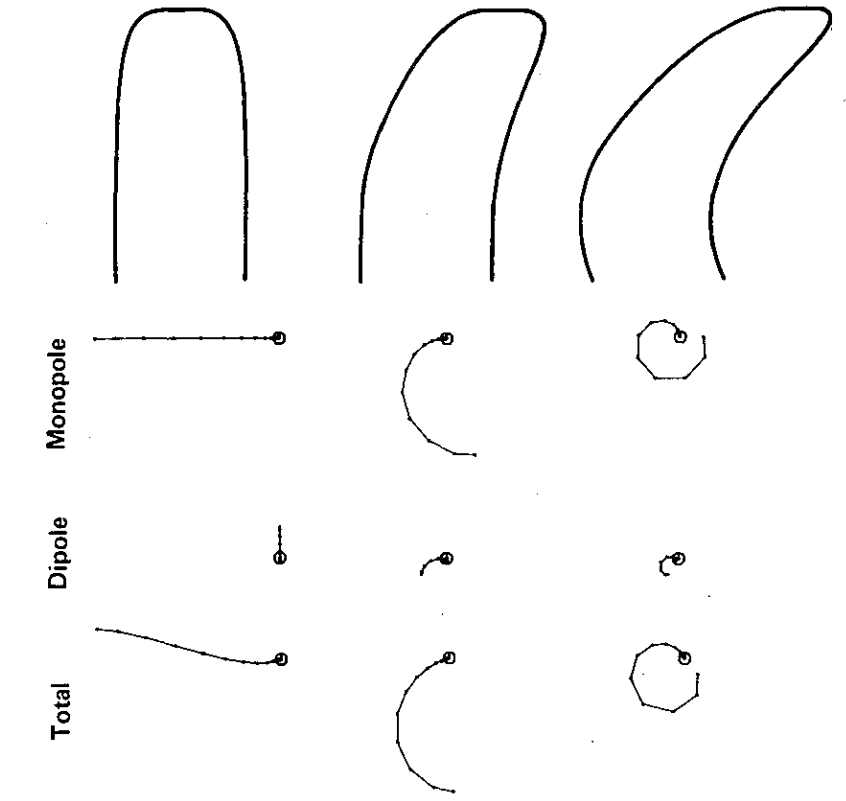
\includegraphics[width=0.5\textwidth]{hasonsweep.png}
    \caption{Example of phase interference for three swept planforms Mx=0.8, MT = 0.822, mB = 8 (vector segments between two dots corresponds to 5\% of blade radius, peak radiation angle = 30 deg).}
    \label{fig:vector_addition}
\end{figure}

The problem for minimising noise of a given harmonic is then to sweep the blade in such a way that minimises the sum of these noise vectors.
The magnitudes of the vectors will be assumed fixed ie constant thickness and loading.


\section{Superposition of Propellers with Even Blade Spacing}

Dobrzynski \cite{uneven_blade_spacing} showed that the noise from a propeller with uneven blade spacing can be reduced by superposition of two propellers with even blade spacing.

\section{Extension to looped propellers}

\begin{figure}[H]
    \centering
    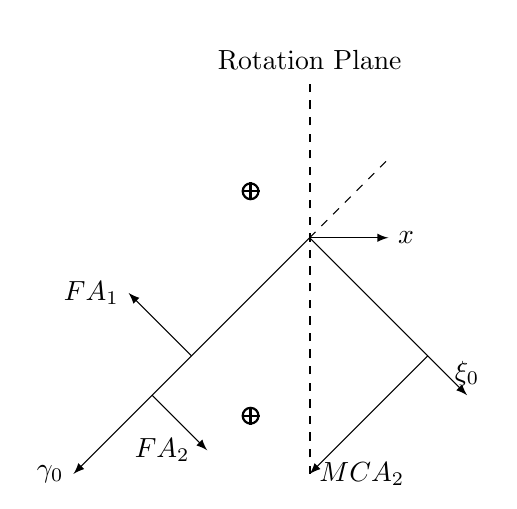
\begin{tikzpicture}
            % Some profiles look better when using plot[smooth]
        \begin{scope}[rotate=225, xshift=-1cm, yshift=-1cm]
            \draw[scale=3,thick=3] node[left=0.5cm] {}
                plot file{../app/foils/NACA2412.surf} -- cycle;
        \end{scope}
        \begin{scope}[rotate=225, xshift=1cm, yshift=1cm]
            \draw[scale=3,thick=3] node[left=-0.5cm] {}
                plot file{../app/foils/NACA2412.surf} -- cycle;
        \end{scope}
        % hoirzontal line
        \draw[thick, dashed] (0,-3) -- (0, 2) node[above] {Rotation Plane};
        \draw[->] (0,0) -- (1,0) node[right] {$x$};
        \draw[->] (0,0) -- (2,-2) node[above] {$\xi_0$};
        \draw[->] (0,0) -- (-3,-3) node[left] {$\gamma_0$};
        \node[cg] at (-0.75,1-0.41) {};
        \node[cg] at (-0.75,1-0.41-3+0.15) {};
        \draw[dashed] (0,0) -- (1,1) node[] {};

        \draw[->] (-1.5,-1.5) -- (-2.5+0.2,-0.5-0.2) node[left] {$FA_1$};
        \draw[->] (-2,-2) -- (-2 + 0.5+0.2,-2.5-0.2) node[left, xshift=-0.1cm] {$FA_2$};
        \draw[->] (1.5,-1.5) -- (-1.5+1.5,-1.5-3+1.5) node[right] {$MCA_2$};
    
    \end{tikzpicture}
    \caption{Local section of propeller blade for BEM. Anticlockwise angles are positive.}
    \label{fig:waffler}
\end{figure}

This means an extended generalised source function can be formed

\begin{equation}
    \begin{aligned}
        g(\eta, r_0, \xi_0) = \rho_0 U^2 \frac{\partial^2 }{\partial \eta^2} &\bigg[ h_1(\eta, r_0)\delta(FA_1 + \xi_0) + h_2(\eta, r_0) \delta(FA_2 + \xi_0)\bigg] \\
        + \frac{\partial }{\partial \boldsymbol{\gamma}_i} &\Big[ f_{1,i}(\eta, r_0) \delta(FA_1 + \xi_0) + f_{2,i}(\eta, r_0) \delta(FA_2 + \xi_0)\Big] \\
    \end{aligned}
    \label{eq:generalised_source_extended}
\end{equation}
All of the operations performed are linear so the far field harmonic
\begin{equation}
    g(\eta, r_0, \xi_0) = g_1(\eta, r_0, \xi_0) + g_2(\eta, r_0, \xi_0)
\end{equation}
Which has respective Fourier transforms $\psi_1$ and $\psi_2$.
\begin{equation}
    P_{mB} = P^{(1)}_{mB} + P^{(2)}_{2mB}
\end{equation}



\begin{thebibliography}{9}

    \bibitem{goldstein_aeroacoustics}
    Goldstein, M. E., 
    \emph{Aeroacoustics},
    McGraw-Hill Book Co., New York, 1976.

    \bibitem{uneven_blade_spacing}
    W. Dobrzynski,
    \emph{Propeller noise reduction by means of unsymmetrical blade spacing},
    Journal of Sound and Vibration, 1991.


\end{thebibliography}

\end{document}
